% sections/04_monitor.tex
\subsection{Monitor: Game Development Environment}
\label{sec:monitor}

The browser-based monitor distinguishes PYNQcast as a \emph{game development environment}.  Commands are published via HTTP POST to Redis Pub/Sub (\texttt{game:control}); T2 subscribes and drains the control queue each tick. Figure~\ref{fig:dashboard} shows some standout panels: (1)~the map editor with brush, fill, and spawn tools for designing 32$\times$32 arenas; (2)~the map library for live hot-swapping of stored arenas; (3)~the live game top-down view with the new geometry rendered; and (4)~the match archive and replay panel, which can stream stored matches directly to a specific player's screen.

\begin{figure}[h]
  \centering
  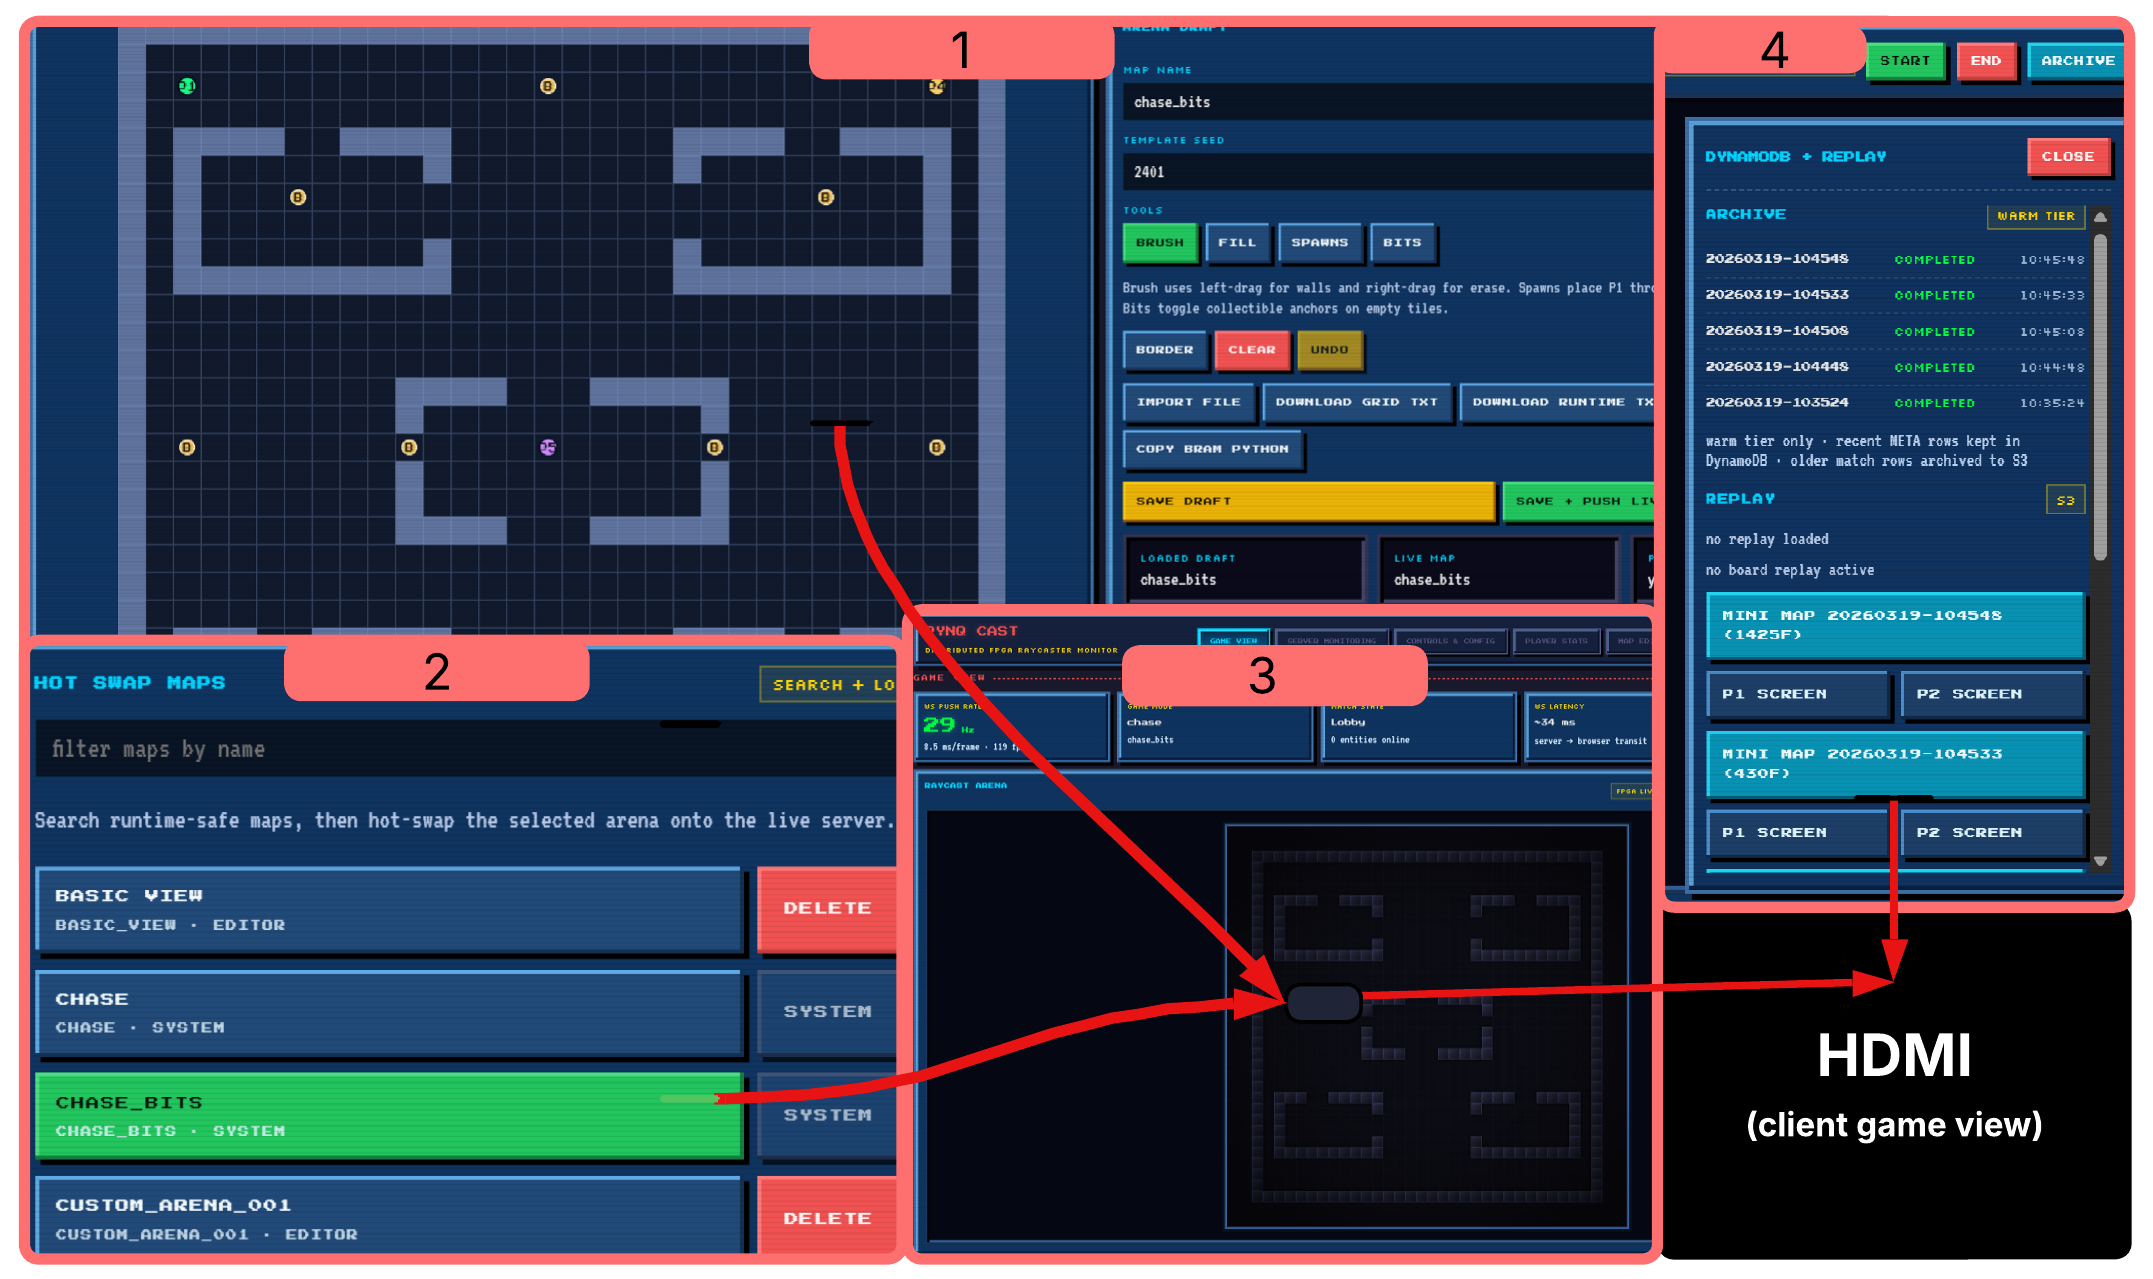
\includegraphics[width=\columnwidth]{images/dashboard_specials.png}
  \caption{Monitor dashboard panes built in HTML, CSS, JS and React. (1)~Map editor (2)~Map library (3)~Live arena with all players (4)~Match Replay activation from S3}
  \label{fig:dashboard}
\end{figure}

 Every match is automatically recorded via the sidecar's S3 replay stream; ``P1/P2 Screen'' button fetches the file, switches target boards into replay mode via \texttt{PKT\_NODE\_MODE}, and streams each frame as a standard \texttt{PKT\_GAME\_STATE} at the original tick rate. The FPGA re-executes original game geometry from stored state.
